\mychapter{Credential Relationship Binding Nullifier}

\section{Introduction}

In Chapters 2 and 3, we developed a robust foundation for anonymous credentials, evolving from single-issuer Attribute-Based Anonymous Credentials $(\ABC)$ to the Multi-Issuer Multi-Credential ABC $(\MIMCABC)$ system with identity binding security. $\MIMCABC$ enables users to privately prove that credentials from multiple, mutually distrusting issuers belong to the same identity, a significant advance for applications like federated identity proofs or content credentialing. However, real-world identity systems impose additional requirements that $\MIMCABC$ does not fully address: hierarchical structure and sybil resistance for context-specific credentials.

In practice, credentials often form a natural hierarchy, with foundational identities—such as government-issued IDs or passports—serving as Master Credentials, and dependent credentials—like driver’s licenses, professional certificates, or access rights—acting as Context Credentials. This structure enables efficient revocation: invalidating a Master Credential (e.g., upon employment termination) implicitly revokes all dependent Context Credentials, avoiding the need to track and revoke each individually. Furthermore, regulatory frameworks like KYC/AML demand accountability, requiring systems to prevent sybil attacks where users illegitimately obtain multiple credentials for the same context (e.g., multiple driver’s licenses). 

While MIMC-ABC ensures credentials share a single identity, it lacks mechanisms to enforce this hierarchical dependency or prevent sybil attacks in a privacy-preserving manner, as its identity binding operates agnostically across all credentials without distinguishing their roles or contexts. To meet these practical and regulatory needs, we must extend MIMC-ABC with a cryptographic framework that organizes credentials hierarchically and ensures context-specific uniqueness, all while preserving user anonymity and computational efficiency


\subsection{Background Work}

Past works tackled hierarchy and sybil resistance in credential systems. None fully balances privacy, efficiency, and flexibility. 
\begin{enumerate}
    \item The UTT anonymous payment system ~\cite{tomescu2022utt} is the closest work, using a registration credential (like a Master Credential) and the coins are also credentials using serial numbers (like Context Credentials) where a coin can only be spent once. UTT uses pairings in their pseudorandom function which we benchmark against.

    \item CanDID~\cite{maram2021candid} defines Master and Context Credentials clearly, but has weakened privacy. It uses mappings between credential public keys in a table, breaking unlinkability. It also relies on an MPC-based PRF for sybil resistance. This adds complexity and overhead, unfit for lightweight use.

    \item Other pairing-based systems, like SyRA~\cite{crites_syra_2024} and S3ID~\cite{rabaninejad_attribute-based_2024}, offer private hierarchies. Yet, they suffer from pairing-related efficiency issues. 

    \item Standard Verifiable Random Functions  (VRFs)~\cite{hutchison_verifiable_2005} reveal the user’s public key during verification impact anonymity.

\end{enumerate}


Our MIMC-ABC system (Chapter 3) binds identities efficiently and anonymously but without hierarchy and context-specific sybil resistance. We need a solution that keeps MIMC-ABC’s strengths. It must add a light, private way to handle credential hierarchies and sybil resistance.


\subsection{Problem Statement}

We want to improve MIMC-ABC for real-world use. Our goal is a private credential hierarchy with Sybil resistance. A user has a Master Credential with a secret key $\k$. They also have Context Credentials with unique IDs $\ctx$ (e.g., $\mathcal{H}(\text{"DriverLicense"})$). We need a mechanism that:
\begin{enumerate}
    \item Links each Context Credential to the Master Credential. It uses a unique nullifier $\nul$ from committed values $\k$ and $\ctx$ from different commitments.
    \item Prevents sybil attacks. It prevents multiple nullifiers for the same $(k, \ctx)$ pair.
    \item Verifies nullifier correctness in zero-knowledge. It hides $\k$ and $\ctx$.
\end{enumerate}


Our main challenge is:
\begin{center}
\emph{How do we build an efficient, pairing-free VRF with zero-knowledge proofs? It must generate and verify nullifiers for a hierarchical anonymous credential system under standard assumptions.}
\end{center}

\begin{table}
\begin{center}
\caption{Comparison of our construction over previous work.}
\label{tab:comparison-chap4}
\begin{tabular}{l|ccccc}
Features    									& 
Sybil Resist.  & 
Hierarchy & 
Private & 
Pairing-Free & 
Predicate Proofs \\
\hline
CanDID \cite{maram2021candid}     				&
\ding{51}     & 
\ding{51} 	& 
\ding{55}  &  
-     & 
\ding{55}		\\
SyRA \cite{crites_syra_2024}     				& 
\ding{51}    	& 
\ding{51}     & 
\ding{51}  &  
\ding{51}     & 
\ding{55}		\\
S3ID \cite{rabaninejad_attribute-based_2024}  & 
\ding{51}     & 
\ding{51}    	& 
\ding{55}  &  
\ding{55}     & 
\ding{55}		\\
UTT               & 
\ding{51}     & 
\ding{51}    	& 
\ding{51}  &  
\ding{55}     & 
\ding{51}		\\
Chap3             & 
\ding{55}     & 
\ding{55}    	& 
\ding{51}  &  
\ding{55}     & 
\ding{51}		\\
Ours  										& 
\ding{51}     & 
\ding{51}    	& 
\ding{51}  &  
\ding{51}     & 
\ding{51}		\\
\end{tabular}
\end{center}
\vspace{1em}
\footnotetext[1]{Predicate Proofs allow users to prove statements about their credentials privately}
\footnotetext[2]{Efficient Token refers to optimization of token verification}
\end{table}

\subsection{Contributions}

We advance anonymous credential systems by developing a lightweight, pairing-free Verifiable Random Function (VRF) construction optimized for our use-case of hierarchical credential binding and sybil resistance. Our contributions are threefold:

\begin{enumerate}
        \item \textbf{Pairing-Free VRF in Prime-Order Groups:} We adapt the Dodis-Yampolskiy VRF structure to function efficiently in standard prime-order groups, achieving provable pseudorandomness under the $q$-Diffie-Hellman Inversion ($q$-DHI) assumption. We show that VRF evaluation is 33\% faster and verification is 60\% faster than previous constructions.

        \item \textbf{Novel $\Sigma$-protocol for Multiplicative Inverse:} We show our problem reduces to proving a committed value equals the multiplicative inverse of another committed value and introduce an efficient zero-knowledge proof technique for proving the relation without using pairings. The protocol has value beyond our specific application, offering a new general technique for $\Sigma$-protocols requiring $q-DHI$ relationships.

         \item \textbf{Formal Security Guarantees:} maintains \emph{Pseudorandomness} of the VRF outputs in the indistinguishable outputs, \emph{uniqueness} in one nullifier per $(\k, \ctx)$ pair preventing sybil attacks

\end{enumerate}

Levearging our work, we propose the Credential Relationship Binding Nullifier (CRBN) which extends the MIMC-ABC system into a complete identity framework with benefits:

\begin{enumerate}
    \item Cryptographically binds master credentials (containing key $\k$) to context credentials (with context identifiers $\ctx$) via a verifiable nullifier enabling accountability

    \item Enforces sybil resistance for context credentials while retaining privacy by using committed attributes and zero-knowledge proofs

    \item Integrates with the efficient $\Sigma$-protocols used throughout the system
    
\end{enumerate}















\section{Preliminaries}
\subsection{Cryptographic Assumptions}

\begin{definition}[q-DHI Assumption]
Let $\mathbb{G}$ be a cyclic group of prime order $p$ with generator $g$. The $q$-Diffie-Hellman Inversion ($q$-DHI) assumption \cite{mitsunari_new_2002} states that for any PPT adversary $\mathcal{A}$, there exists a negligible function $\negl$ such that:
\[
\Pr\left[ x \sample \Zp^*, \quad \mathcal{A}(g, g^x, g^{x^2}, \ldots, g^{x^q}) = g^{1/x} \right] \leq \negl 
\]
where the probability is taken over the random choice of $x$ and the random coins of $\mathcal{A}$. Informally, no $\PPT$ adversary can distinguish between $g^{1/\alpha}$ from a random group element.
\end{definition}

\begin{remark}
The $q$-DHI assumption is equivalent to the $(q+1)$-generalized Diffie-Hellman assumption (GDH) as shown by Boneh and Boyen \cite{kanade_efficient_2004}. This equivalence provides a solid theoretical foundation for the security of our VRF construction.
\end{remark}


\subsection{Building Blocks}
We use the Pedersen Commitments from chapter 2, committing to a vector of messages $\cm = \CMCom([\id, \ctx, \exp, \k];\usk) = g_1^\id g_2^\ctx g_3^\exp g_4^\k g^\usk$. Pedersen Commitments are hiding, binding, and position-binding which enforces their position in the vector of messages such that the exponent at one position can't be swapped with another position. 

We use the three-move $\Sigma$-protocols \ref{preliminaries-sigmaprotocol} to prove relations of exponents which we represent as $\mathcal{R}_{\mathsf{VRF}} = \left\{(w)(x) \mid x = g^w \right\}$ proving knowledge of secret witness $w$ with public statement $x$. 


\begin{definition}[Verifiable Random Function]
A Verifiable Random Function (VRF) is a tuple of probabilistic polynomial-time algorithms $(\PPT)$ $(\mathsf{VRF.Gen}, \mathsf{VRF.Eval}, \mathsf{VRF.Vfy})$ with an associated message space $\setX$, output space $\setY$ and proof space $\Pi$ defined as:
\begin{itemize}
    \item $\mathsf{VRF.Gen}(1^\lambda) \to (sk, pk)$: Takes a security parameter $\lambda$ and outputs a secret key $sk$ and a public key $pk$.
    
    \item $\mathsf{VRF.Eval}(sk, x) \to (y, \pi)$: On input $x \in \setX$ and secret key $sk$, outputs a value $y \in \setY$ and a proof $\pi \in \Pi$.
    
    \item $\mathsf{VRF.Vfy}(pk, x, y, \pi) \to \{0,1\}$: Using the public key $pk$, verifies that $y$ is the correct output for input $x$ with proof $\pi$, returning 1 if valid, 0 otherwise.
\end{itemize}
    
\end{definition}
A $\VRF$ must satisfy three properties
\begin{itemize}
    \item \textbf{Correctness:} For all $(sk, pk) \gets \mathsf{VRF.Gen}(1^\lambda)$ and all $x \in \setX$:
    \[
    \Pr\left[\begin{aligned}
        (y, \pi) &\gets \mathsf{VRF.Eval}(sk, x) \\
        1 &\gets \mathsf{VRF.Vfy}(pk, x, y, \pi)
    \end{aligned}\right] = 1
    \]

    \item \textbf{Unique Provability:} For any $pk$ (possibly malicious) and $x \in \setX$, no $\PPT$ adversary $\AdvA$ can find two distinct pairs of outputs $(y_0, \pi_0) \neq (y_1, \pi_1)$ such that:
    \[
    \mathsf{VRF.Vfy}(pk, x, y_0, \pi_0) = \mathsf{VRF.Vfy}(pk, x, y_1, \pi_1) = 1
    \]

    \item \textbf{Pseudorandomness:} Informally, this property ensures that without the secret key, the output of the VRF for an unqueried input is indistinguishable from a random value, even when the adversary can see other input-output pairs.
    Formally, For any PPT adversary $\mathcal{A}$, the advantage in the following experiment is negligible:
    \[
    \left|\Pr\left[\begin{array}{l}
        (sk, pk) \gets \mathsf{VRF.Gen}(1^\lambda) \\
        x^* \gets \mathcal{A}^{\mathcal{O}_{\mathsf{VRF.Eval}(sk, \cdot)}}(pk) \\
        (y^*, \pi^*) \gets \mathsf{VRF.Eval}(sk, x^*) \\
        y_0 \gets y^*; \, y_1 \sample \mathcal{Y} \\
        b \sample \{0,1\} \\
        b' \gets \mathcal{A}^{\mathcal{O}_{\mathsf{VRF.Eval}(sk, \cdot)}}(pk, y_b)
    \end{array} : b' = b \wedge x^* \notin \mathcal{Q}\right] - \frac{1}{2}\right| \leq \negl(\lambda)
    \]
    where the oracle $\mathcal{O}_{\mathsf{VRF.Eval}(sk, \cdot)}$ takes input $x \in \mathcal{X}$ (where $x \neq x^*$) and outputs $(y, \pi) \gets \mathsf{VRF.Eval}(sk, x)$. $\mathcal{Q}$ is the set of oracle queries made to $\mathcal{O}_{\mathsf{VRF.Eval}(sk, \cdot)}$  
\end{itemize}





\section{Construction}
We develop a novel Verifiable Random Function (VRF) construction from committed attributes and show how it supports our anonymous credential hierarchy requirements. At the core is our novel zero-knowledge proof protocol to prove two committed attributes are multiplicative inverse of each other which is of independent interest. 

\subsection*{Notation}
Inline with our Anonymous Credential scheme built and prior chapters, the secret key is $\k$, the VRF input is $\ctx$, the VRF output is $\nul$ and the proof $\pi$ proves the correctness of $\nul$ such that $(\nul, \pi) \gets \mathsf{VRF.Eval}(\k, \ctx)$. $\cm = \CMCom([\id,\ldots];\usk)$ is a commitment shorthand for commitment $g_1^\id \ldots g^\usk$

\subsection*{Roadmap}
We start with the classical Dodis-Yampolskiy VRF \cite{hutchison_verifiable_2005} and introduce step-changes to adapt it for privacy and efficiency. The nullifier format $\nul = g^{1/(\k+\ctx)}$ remains the same throughout as the proof $\pi$ changes shape.
\begin{enumerate}
    \item \textbf{Dodis-Yampolskiy VRF with Bilinear Pairings}: We begin with revisiting the classical Dodis-Yampolskiy VRF using bilinear pairings where 
    $pk = g^\k$ is public, $\ctx$ is public, $\k$ is secret. $\VRFEval$ outputs $\nul$ and proof $\pi = e(g_1, g_2)^{1/(\k + \ctx)}$
    
    \item \textbf{Prime-Order Group VRF}: We then adapt the VRF to a prime-order group setting while retaining the security properties under $q$-DHI. We run a $\Sigma$-protocol to generate the proof $\pi$ attesting to the relation, noting that $\pk$ and $\ctx$ are public and used in verification

    \[
    \Rel = \zkpok \left\{(pk, \ctx, \nul, \n) (\k) \mid \nul = g^{1/(\k + \ctx)} \quad \wedge \quad \n =  pk \cdot g^x  \right\}
    \]
    
    \item \textbf{VRF with Committed Inputs}: Next, we hide the secret key $\k$ and context identifier $\ctx$ in a commitment $\cm = \CMCom([\k, \ctx]; \usk)$ and show the proof $\pi$ attesting to the relation, noting the commitment is public but $\ctx$ is hidden

    \[
    \Rel = \zkpok \left\{ (\nul, \cm)(\k, \ctx) \mid \nul = g^{1/(\k + \ctx)} \quad \wedge \quad \cm = g_1^\k g_2^{\ctx}g^r  \right\}
    \]

    \item \textbf{VRF from (multiple) Committed Inputs for $\MIMCABC$}: Finally, we extend the $\Sigma$-protocol to incorporate our Anonymous Credential requirements. We derive the nullifier from two separate commitments, $\cmm = \CMCom([\id, \ctx_m, \exp_m, \k_m]; \usk_m)$ from the master credential and $\cmc = \CMCom([\id, \ctx_c, \exp_c]; \usk_c)$ from the context credential. The relation proves the following 
    \begin{enumerate}
        \item prover can open $\cmm$ and its from a Master Credential and contains the $\k_m$ we're using %$\ctx=\texttt{master}$
        \item prover can open $\cmc$ and its from a Context Credential
        \item The derived nullifier is correct $\nul = g^{1/(\k_m + \ctx_c)}$ 
    \end{enumerate}
    
    \[
        \mathcal{R}_{\mathsf{vrf}} = \zkpok \left\{ 
        \begin{array}{l} 
        (\cmm, \cmc, \mathsf{N}), (\id, \ctx, , \exp, \k, r_1, r_2) \\
        \end{array} 
        \middle|
        \begin{array}{l}
            \cmm = g_1^{\id}g_2^{\ctx_m}g_3^{\exp_m}g_4^{\k_m}g^{r_m}  \wedge \ctx=\texttt{master} \\
            \cmc = g_1^{\id}g_2^{\ctx_c}g_3^{\exp_c}g^{r_c} \wedge \ctx=\texttt{dmv} \\
            \nul = g^{1/(k_m + \ctx_c)}
        \end{array} 
        \right\}
    \]

\end{enumerate}




\subsection{Dodis-Yampolskiy VRF with Bilinear Pairings}
We begin by revisiting the Dodis-Yampolskiy VRF, defined in a bilinear group setting (we use Type-3 pairings). Let $\G_1$, $\G_2$, and $\G_T$ be groups of prime order $p$, with generators $g \in \G_1$, $\tilde{g} \in \G_2$, and a bilinear map $e: \G_1 \times \G_2 \to \G_T$.

The VRF is specified as:
\begin{itemize}
    \item $\mathsf{VRF.Gen}(1^\lambda)$: Sample $\k \sample \mathbb{Z}_p^*$ and compute $pk = g_1^\k$. Output $(\k, pk)$.
    \item $\mathsf{VRF.Eval}(\k, \ctx) \to (\nul, \pi)$: compute: $\nul = \tilde{g}^{1/(\k + \ctx)}$, $\pi = e(g, \tilde{g})^{1/(\k + \ctx)}$ for $\ctx \in \Z_p$
    \item $\mathsf{VRF.Vfy}(pk, \ctx, \nul, \pi) \to \{0, 1\}$: Assert: $e(g^\ctx \cdot pk, \nul) \stackrel{?}{=} e(g, \tilde{g}) \quad $ and $\quad \pi \stackrel{?}{=} e(g, \nul)$
\end{itemize}

The $\mathsf{Eval}$ function generates a nullifier $\mathsf{N}$ and a proof $\pi$, enabling anyone with $pk$ and $\textsf{ctx}$ to verify that $\mathsf{N}$ was computed correctly. The verification mimics a signature check, binding $pk$, $\textsf{ctx}$, and $\mathsf{N}$.

\textbf{Verification Details:}

1. \textbf{First Pairing Equation:}
   \[
   e(g_1^{\textsf{ctx}} \cdot pk, \mathsf{N}) = e(g_1^{\textsf{ctx}} \cdot g_1^k, g_2^{1/(k + \textsf{ctx})}) = e(g_1^{\textsf{ctx} + k}, g_2^{1/(k + \textsf{ctx})}) = e(g_1, g_2)^{(\textsf{ctx} + k)/(k + \textsf{ctx})} = e(g_1, g_2)^1 = e(g_1, g_2).
   \]
   This confirms $\mathsf{N}$'s consistency with $pk$ and $\textsf{ctx}$.

2. \textbf{Second Pairing Equation:}
   \[
   \pi = e(g_1, g_2)^{1/(k + \textsf{ctx})}, \quad e(g_1, \mathsf{N}) = e(g_1, g_2^{1/(k + \textsf{ctx})}) = e(g_1, g_2)^{1/(k + \textsf{ctx})},
   \]
   so $\pi = e(g_1, \mathsf{N})$, binding the proof to $\mathsf{N}$.

\subsubsection{Informal Security Analysis}
\begin{itemize}
    \item \textbf{Correctness}: The pairing properties ensure that honestly computed $\mathsf{N}$ and $\pi$ satisfy the verification equations.
    \item \textbf{Unique Provability}: For each $\textsf{ctx}$, only $\mathsf{N} = g_2^{1/(k + \textsf{ctx})}$ satisfies $e(g_1^{\textsf{ctx}} \cdot pk, \mathsf{N}) = e(g_1, g_2)$. Forging a different $\mathsf{N}'$ requires solving the discrete logarithm problem, which is intractable.
    \item \textbf{Pseudorandomness}: The output $\mathsf{N}$ appears random under the $q$-Diffie-Hellman Inversion ($q$-DHI) assumption. Given $g_1, g_1^k, \ldots, g_1^{k^q}$, distinguishing $\mathsf{N} = g_2^{1/(k + \textsf{ctx})}$ from a random $\mathbb{G}_2$ element reduces to computing $g_2^{1/k}$, a hard $q$-DHI instance.
\end{itemize}













Notes below! 





\section{Construction 1. VRF in prime-order group}
Our Verifiable Random Function (VRF) works in a prime-order group $\G$ with generator $g$, where the evaluation outputs $y = g^{1/(sk + x)}$ for an input $x$ and secret key $sk$, and the verification protocol shows that $y^{sk + x} = g$.

\subsection{VRF Construction}
Our VRF operates in a prime-order group $\mathbb{G}$ of order $p$ with generator $g$. Define the message space $\setX = \mathbb{Z}_p$, output space $\setY = \mathbb{G}$, and proof space $\Pi = \mathbb{G} \times \mathbb{G} \times \mathbb{Z}_p$. 
\begin{itemize}
    \item $\VRFGen(1^\lambda) \to (sk, pk)$:  
    Sample $sk \sample \mathbb{Z}_p^*$, compute $pk = g^{sk}$, and output $(sk, pk)$.
    \item $\VRFEval(sk, x) \to (y, \pi)$:  
    Compute $y = g^{1/(sk + x)}$.  
    To generate $\pi$:  
    \begin{enumerate}
        \item \textbf{Commitment}: $\mathcal{P}$ Samples $r \sample \Z_q$. Computes $T_1 = g^r$, $T_2 = y^r$
        \item \textbf{Challenge}: $\mathcal{V}$ sends challenge $c$
        \item \textbf{Response}: $\mathcal{P}$ Computes $z= r + c \cdot (sk + x)$. Sets $\pi = (T_1, T_2, z)$
    \end{enumerate}
    \item $\VRFVfy(pk, x, y, \pi, st) \to \bit:$ retrieve $c$ from state $st$. Parse $\pi = (T_1, T_2, z)$, compute $C = pk \cdot g^x$, verify
    \[
        g^z = T_1 \cdot C^c \quad \wedge \quad y^z = T_2 \cdot g^c
    \]
\end{itemize}
This construction satisfies the VRF properties - correctness, uniqueness, and pseudorandomness under the under the $q$-DHI assumption. Note that we use a public key $pk$ and VRF input $x$ which are both public. 

\subsubsection{Comparison to Dodis-Yampolskiy VRF}
The Dodis-Yampolskiy VRF also evaluates $y = g^{1/(sk + x)}$, but relies on a bilinear group for the proof $\pi$ using a pairing check: $e(y, pk \cdot g^x) = e(g, g)$, which is computationally heavy. Our construction sticks to the prime-order group, proves $y^{sk + x} = g$ with a $\Sigma$-protocol.






\section{Construction 2. VRF from commitment exponents}

Let's show that a commitment $cm = g_1^sk g_2^x g^r$ can in privacy produce the VRF.
Such that $y = g^{1/x + sk}$ and $\pi$ proves that  $y^{sk + x} = g$.


















































% Introduce Pedersen commitments, VRFs, $\Sigma$-protocols

\subsection{Notation}
% Define $\mathbb{G}$, $p$, $g$, $\mathsf{CM.Com}$, etc.

\section{Nullifier Construction}
\subsection{Intuition}
% High-level overview: purpose, why pairing-free matters
% 

\subsection{Formal Definition}
% Define $\nul = g^{1/(\k + \ctx)} \in \mathbb{G}$

\subsection{Algorithms}
% Nullifier generation: how $\nul$ is computed
% Verification: sketch of zero-knowledge check

\subsection{Properties}
% List $Uniqueness$, $Pseudorandomness$, $Zero-Knowledge$

\section{Protocol for Nullifier Verification}
\subsection{Overview}
% Goal: prove $\nul$ correctness without revealing $\k$, $\ctx$

\subsection{Commitment Structure}
% Master: $\cmm = g_1^\id g_2^{\ctx_m} g_3^{\exp_m} g_4^\k g^{r_m}$
% Context: $\cmc = g_1^\id g_2^{\ctx_c} g_3^{\exp_c} g^{r_c}$

\subsection{$\Sigma$-Protocol}
% Define $\mathcal{R}_{\mathsf{vrf}} = \{ ... | \nul = g^{1/(\k + \ctx_c)} \}$


\subsection{Efficiency}
% Highlight pairing-free advantage






\section{Integration into MIMC-ABC}
\subsection{Modified Algorithms}
% Issuance: Master/Context credential setup
% Presentation: $\nul$ proof with MIMC-ABC

\subsection{Revocation and Sybil Resistance}
% Revocation: $\cmm$ or $\k$ invalidation
% Sybil Resistance: nullifier registry

\subsection{Example}
% Passport and driver’s license with $\nul$

\section{Security Analysis}
\subsection{Security Model}
% Adversary definition, security games

\subsection{Theorems}
% $Uniqueness$, $Pseudorandomness$, $Zero-Knowledge$ proofs

\subsection{Sybil Resistance}
% Nullifier prevents multiple credentials per context

\section{Performance Evaluation}
\subsection{Benchmarks}
% Compare to pairing-based VRFs: 33\%/60\% speedup

\subsection{Scalability}
% Overhead with increasing credentials

\subsection{Implementation}
% Rust/arkworks details





























\subsection{Construction}
During verification, the user proves in zero-knowledge that they possess a valid master credential with VRF key $\k$, a context credential with a specific $\ctx$ value and the nullifier $\nul$ is correctly formed by using a secret $\k$ in $\credm$ and $\ctx$ in $\credc$. 

\begin{equation}
\nul = g^{1/(\k + \ctx)} \in \G
\end{equation}

\subsection{Integration with Identity System}


\begin{figure}
        \begin{pchstack}[boxed, center, space=4em]
            \begin{pcvstack}
                \procedure[space=auto]{Passport}{%
                \id: 12345, \\
                \ctx: "master", \\
                \exp: "10/11/2026" \\
                \k: 54321
                }
            \end{pcvstack}
            \pcvspace
            \begin{pcvstack}
                \procedure[space=auto]{Driver License}{%
                 \id: 12345, \\
                 \ctx: "DMV", \\
                 \exp: "10/11/2028"
                }
            \end{pcvstack}
            \begin{pcvstack}
                \procedure[space=auto]{Nullifier}{%
                 \textsf{n} = 1/(\k + "DMV") \\
                 \nul = g^{\textsf{n}}
                }
            \end{pcvstack}
        \end{pchstack}
    \caption{Example Credential and Nullifier for context DMV}
    \label{fig:two-creds}
\end{figure}


\[
    \mathcal{R}_{\mathsf{vrf}} = \zkpok \left\{ 
    \begin{array}{l} 
    (\cmm, \cmc, \mathsf{N}), (\id, \ctx, , \exp, \k, r_1, r_2) \\
    \end{array} 
    \middle|
    \begin{array}{l}
        \cmm = g_1^{\id}g_2^{\ctx}g_3^{\exp}g_4^{\k}g^{r_1}  \wedge \ctx="master" \\
        \cmc = g_1^{\id}g_2^{\ctx}g_3^{\exp}g^{r_2} \wedge \ctx="DMV" \\
        \nul = g^{1/(k + \ctx)}
    \end{array} 
    \right\}
\]
    

This requires only standard group operations and leverages the proof machinery already present in our credential system, avoiding the computational cost of pairings.




\subsection{Security Properties}
Our nullifier construction provides:

\begin{itemize}
    \item \textbf{Uniqueness}: For fixed $\k$ and $\ctx$, the nullifier is deterministic and unique
    \item \textbf{Unlinkability}: Nullifiers for different contexts are unlinkable without knowledge of $\k$
    \item \textbf{Double-spending prevention}: The system can detect if the same user attempts to obtain multiple credentials for the same context
\end{itemize}

These properties follow directly from the security of our underlying commitment scheme and the algebraic properties of the multiplicative inverse. The formal security analysis extends our existing credential system model.



\subsection{Zero-Knowledge Proof of Multiplicative Inverse}
The core technical challenge in our construction is proving knowledge of $\k$ and $\ctx$ (from different commitments) such that $\nul = g^{1/(\k + \ctx)}$ without revealing these values, we do this by introducing an auxiliary variable $\n = 1/(\k + \ctx) \in \Z_p$ and proving that $\n \cdot (\k + \ctx) = 1 \quad \wedge \quad \nul = g^z$

Our $\Sigma$-protocol for this relation works as follows:

\begin{protocol}{Non-Pairing VRF Output Verification}{non-pairing-vrf-verify}\label{pok-non-pairing-vrf}
\textbf{Common Input:} Group generators $g_1, g_2, g_3, g_4, g_5, g \in \mathbb{G}$, and commitments $\cm_1, \cm_2, \cm_3, \cm_4, \cm_5, \cm_6 \in \mathbb{G}$\\
\textbf{Prover Input:} Witness $(\id, \k, \ctx, r_1, r_2, r_3, r_4, r_5, \textsf{n}, r_6)$ such that:
    \begin{align*}
        \cm_1 &= g_1^{\id} g_2^{\k} g^{r_1}     &    \cm_2 &= g_1^{\id} g_3^{\ctx} g^{r_2}  &   \cm_3 &= g_4^{\k + \ctx} g^{r_3}\\
        \cm_4 &= g_5^{\textsf{n}} g^{r_4}   &   \cm_5 &= \cm_3^{\textsf{n}} g^{r_5}     &   \cm_6 &= g^{r_6} \\
        \textsf{n} &= \frac{1}{\k + \ctx}   &   r_6 &= r_3 \cdot \textsf{n} + r_5    &   \frac{\cm_5}{\cm_6} &= g_4
    \end{align*}

\begin{enumerate}
    \item \textbf{Commitment:} Prover samples random blinding factors from $\Z_q$:
    \[
        a_x \quad \text{ for } \quad x \in \{\ \id, \k, \ctx, \textsf{n}, r_1, \ldots,r_6\} \in \Z_q
    \]
    \textbf{Computes}:
    \begin{align*}
        T_1 &\gets g_1^{a_{\id}} g_2^{a_k} g^{a_{r_1}}  &   T_2 &\gets g_1^{a_{\id}} g_3^{a_{\ctx}} g^{a_{r_2}}     &   T_3 &\gets g_4^{a_k + a_{\ctx}} g^{a_{r_3}} \\
        T_4 &\gets g_5^{a_{\textsf{n}}} g^{a_{r_4}}   &   T_5 &\gets \cm_3^{a_{\textsf{n}}} g^{a_{r_5}}     &   T_6 &\gets g^{a_{r_6}}
    \end{align*}
    Sends $(T_1, T_2, T_3, T_4, T_5, T_6)$ to verifier.
    
    \item \textbf{Challenge:} Verifier samples $c \sample \mathbb{Z}_q$ and sends to prover.
    
    \item \textbf{Response:} Prover computes:
    \[
    z_x = a_x + c \cdot x \quad \text{ for } \quad x \in \{\ \id, \k, \ctx, \textsf{n}, r_1, \ldots,r_6\} 
    \]
    Sends $(z_{\id}, z_k, z_{\ctx}, z_{r_1}, z_{r_2}, z_{r_3}, z_{\textsf{n}}, z_{r_4}, z_{r_5}, z_{r_6})$ to verifier.
    
    \item \textbf{Verification:} Verifier checks:
    \begin{align*}
        g_1^{z_{\id}} g_2^{z_k} g^{z_{r_1}} &\stackrel{?}{=} T_1 \cdot \cm_1^c 
        & 
        g_1^{z_{\id}} g_3^{z_{\ctx}} g^{z_{r_2}} &\stackrel{?}{=} T_2 \cdot \cm_2^c \\
        g_4^{z_k + z_{\ctx}} g^{z_{r_3}} &\stackrel{?}{=} T_3 \cdot \cm_3^c
        &
        g_5^{z_{\textsf{n}}} g^{z_{r_4}} &\stackrel{?}{=} T_4 \cdot \cm_4^c \\
        \cm_3^{z_{\textsf{n}}} g^{z_{r_5}} &\stackrel{?}{=} T_5 \cdot \cm_5^c
        &
        g^{z_{r_6}} &\stackrel{?}{=} T_6 \cdot \cm_6^c
        &
        \frac{\cm_5}{\cm_6} &\stackrel{?}{=} g_4
    \end{align*}
\end{enumerate}
\end{protocol}

\section{Proofs}

Theorem: Correctness

Theorem: Soundness

Theorem: Zero Knowledge

\section{Security}

Our nullifier construction builds on the Dodis-Yampolskiy VRF \cite{hutchison_verifiable_2005}, adapting it to work efficiently in standard prime-order groups without pairings. The security relies on the $q$-Diffie-Hellman Inversion ($q$-DHI) assumption, which states that given $(g, g^x, g^{x^2}, \ldots, g^{x^q})$, no PPT adversary can compute $g^{1/x}$ with non-negligible probability \cite{mitsunari_new_2002}.

\subsubsection{Security Properties}

Our nullifier construction satisfies three critical security properties:

\begin{itemize}
    \item \textbf{Uniqueness}: For fixed $\k$ and $\ctx$, the nullifier $\nul = g^{1/(\k + \ctx)}$ is deterministic, ensuring each user can generate exactly one nullifier per context. This prevents Sybil attacks where users attempt to obtain multiple credentials for the same context.
    
    \item \textbf{Pseudorandomness}: Without knowledge of $\k$, the nullifier $\nul$ is computationally indistinguishable from a random group element under the $q$-DHI assumption. This ensures that nullifiers cannot be predicted or linked to other user activities.
    
    \item \textbf{Zero-knowledge}: Our $\Sigma$-protocol proves nullifier correctness without revealing any information about $\k$ or $\ctx$, maintaining user privacy while enabling Sybil resistance.
\end{itemize}

The security of our construction follows directly from: (1) the hardness of the $q$-DHI problem in prime-order groups, (2) the correctness and soundness of our multiplicative inverse $\Sigma$-protocol, and (3) the security of our underlying commitment scheme, which ensures the binding of user credentials to their VRF key $\k$.



\subsection{Performance Analysis}
Benchmarks were performed on MacBook Air M2 16GB RAM using our Rust implementation with the arkworks library \cite{arkworks_contributors_arkworks_2022}. Compared to the state-of-the-art nullifier scheme from \cite{tomescu2022utt}, our scheme removes a pairing with a speedup of 33\% for VRF evaluation and 60\% for Verify.

\begin{table}[h!]
\centering
\label{tab:cred-rel-binding-nullifier-table}
\begin{tabular}{l@{\hspace{1.5em}}r@{\hspace{1.5em}}r@{\hspace{1.5em}}r}
\toprule
Operation & Pairing (ms) & Us (ms) & Our Speedup (\%)) \\
\midrule
Evaluate & 5.83 & 3.89 & 33.26 \\
Verify & 6.37 & 2.52 & 60.42 \\
\bottomrule
\end{tabular}
\caption{Credential Relationship Binding Nullifier Scheme Comparison}
\end{table}
\vspace{-1cm}
\begin{figure}[h!]
    \centering
    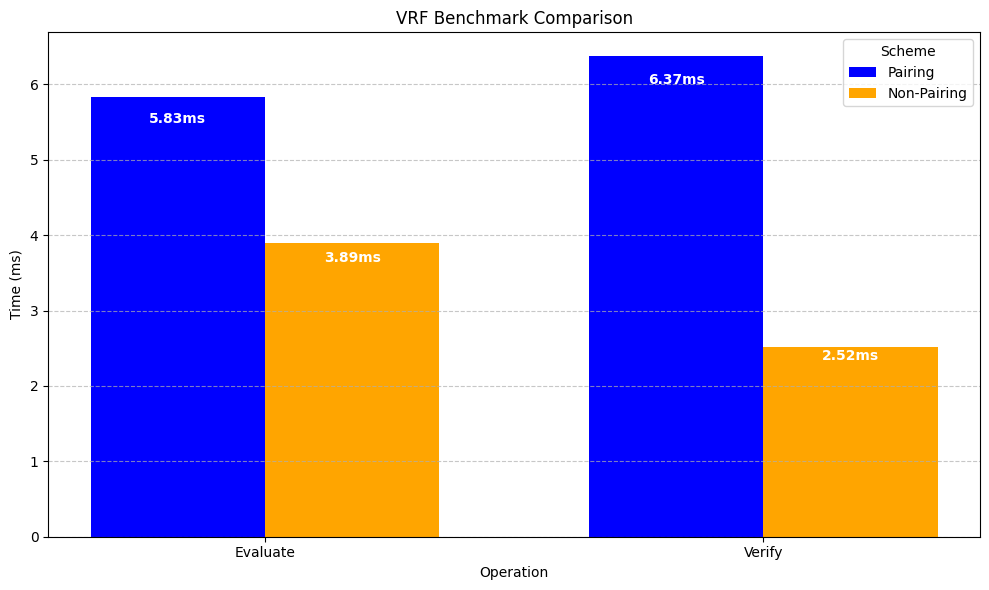
\includegraphics[width=0.75\linewidth]{figures/vrf-benchmark.png}
    \caption{VRF Benchmark}
    \label{fig:vrf-benchmark}
\end{figure}








% \subsection{Construction}

% The Credential Relationship Binding Nullifier (CRBN) extends the Multi-Issuer Multi-Credential Anonymous Credential (MIMC-ABC) system from Chapter 3 to support a hierarchical structure with sybil resistance. We define two credential types: a \emph{Master Credential} containing a secret key $\k$, and \emph{Context Credentials} with context identifiers $\ctx$. A nullifier $\nul = g^{1/(\k + \ctx)} \in \G$ binds each Context Credential to the Master Credential, ensuring uniqueness per context while preserving privacy via zero-knowledge proofs.

% We modify MIMC-ABC’s algorithms as follows, reusing its position-binding Pedersen commitments and $\Sigma$-protocols. Let $\mathsf{pp}$ include $\G$, $p$, $g$, and commitment generators $(g_1, g_2, g_3, g_4, g)$, where $\ell = 4$ supports attributes $[\id, \ctx, \exp, \k]$ (extensible to more).

% \begin{itemize}
%     \item \textbf{Master Credential Issuance}:
%     \begin{itemize}
%         \item \emph{User}: Samples $\k \sample \Z_p$ and $\usk_m \sample \Z_p$. Computes commitment $\cmm = g_1^\id g_2^{\ctx_m} g_3^{\exp_m} g_4^\k g^{\usk_m}$, where $\ctx_m = \mathcal{H}(\text{"master"})$ and $\exp_m$ is the expiration. Runs $\mathsf{Obtain}(\attrs_m = [\id, \ctx_m, \exp_m, \k], \{\mathsf{opk}_j\}, \usk_m)$ with issuer $j_m$, proving $\cmm$’s opening via $\pircom$ (Section 2.4.3).
%         \item \emph{Issuer $j_m$}: Verifies the proof, signs $\sigma_m = \mathsf{RS.Sign}(\cmm, \mathsf{osk}_{j_m})$, and returns $\credm = (\sigma_m, \cmm)$ via $\mathsf{Issue}$.
%     \end{itemize}

%     \item \textbf{Context Credential Issuance}:
%     \begin{itemize}
%         \item \emph{User}: For context $\ctx_c$ (e.g., $\mathcal{H}(\text{"DMV"})$), samples $\usk_c \sample \Z_p$. Computes $\cmc = g_1^\id g_2^{\ctx_c} g_3^{\exp_c} g^{\usk_c}$ (no $\k$ here, as it’s from $\credm$). Runs $\mathsf{Obtain}(\attrs_c = [\id, \ctx_c, \exp_c, 0], \{\mathsf{opk}_j\}, \usk_c)$ with issuer $j_c$, proving $\cmc$’s opening and that position 4 is 0.
%         \item \emph{Issuer $j_c$}: Verifies the proof, optionally checks a nullifier registry (see below), signs $\sigma_c = \mathsf{RS.Sign}(\cmc, \mathsf{osk}_{j_c})$, and returns $\credc = (\sigma_c, \cmc)$.
%     \end{itemize}

%     \item \textbf{Nullifier Generation}: Given $\credm$ with $\k$ and $\credc$ with $\ctx_c$, compute:
%     \[
%     \nul = g^{1/(\k + \ctx_c)} \in \G
%     \]
%     where $\k + \ctx_c$ is computed in $\Z_p$, and the inverse $1/(\k + \ctx_c)$ exists with overwhelming probability (as $p$ is prime).

%     \item \textbf{Presentation and Verification}:
%     \begin{itemize}
%         \item \emph{User}: Inputs $\credm$, $\credc$, $\usk_m$, $\usk_c$, and a predicate $\phi$ (e.g., $\ctx_c = \text{"DMV"} \land \exp_c > \text{today}$). Rerandomizes $\credm$ to $(\sigma_m', \cmm')$ and $\credc$ to $(\sigma_c', \cmc')$ using $\Delta_{r_m}, \Delta_{r_c}$ (Section 3.3). Computes $\nul = g^{1/(\k + \ctx_c)}$ and proves:
%         \[
%         \mathcal{R}_{\mathsf{vrf}} = \zkpok \left\{ 
%         (\cmm', \cmc', \nul), (\id, \ctx_m, \exp_m, \k, \usk_m', \ctx_c, \exp_c, \usk_c') 
%         \middle|
%         \begin{array}{l}
%         \cmm' = g_1^\id g_2^{\ctx_m} g_3^{\exp_m} g_4^\k g^{\usk_m'} \land \ctx_m = \mathcal{H}(\text{"master"}) \land \\
%         \mathsf{RS.Ver}(\sigma_m', \cmm', \mathsf{opk}_{j_m}) = 1 \land \\
%         \cmc' = g_1^\id g_2^{\ctx_c} g_3^{\exp_c} g^{\usk_c'} \land \\
%         \mathsf{RS.Ver}(\sigma_c', \cmc', \mathsf{opk}_{j_c}) = 1 \land \\
%         \nul = g^{1/(\k + \ctx_c)} \land \phi(\ctx_c, \exp_c) = 1
%         \end{array} 
%         \right\}
%         \]
%         where $\usk_m' = \usk_m + \Delta_{r_m}$, $\usk_c' = \usk_c + \Delta_{r_c}$. The proof uses the $\Sigma$-protocol from Section 4.x (to be detailed).
%         \item \emph{Verifier}: Checks $\pi$, $\sigma_m'$, $\sigma_c'$, and $\nul$ against $\mathsf{opk}_{j_m}$, $\mathsf{opk}_{j_c}$. Optionally queries a nullifier registry to ensure $\nul$ is unused for $\ctx_c$.
%     \end{itemize}
% \end{itemize}

% \textbf{Note on Revocation}: If $\credm$ is revoked (e.g., via a public revocation list for $\cmm$ or $\k$), verifiers can reject proofs involving $\nul$, as $\k$’s validity underpins $\mathcal{R}_{\mathsf{vrf}}$. Details are deferred to Section 4.y.

% \textbf{Note on Sybil Resistance}: Issuers or verifiers may maintain a context-specific nullifier registry. During issuance, users prove $\nul$’s correctness in zero-knowledge; issuers reject duplicates. Alternatively, verifiers check $\nul$’s uniqueness during presentation, balancing privacy and accountability (see Section 4.z).

% This construction leverages MIMC-ABC’s efficient $\Sigma$-protocols and avoids pairings, using only standard group operations in $\G$. The nullifier $\nul$ enforces hierarchical binding and sybil resistance, computed deterministically from $\k$ and $\ctx_c$.

